\chapter{HASIL DAN PEMBAHASAN}
\label{chap:hasilpembahasan}

% Ubah bagian-bagian berikut dengan isi dari hasil dan pembahasan

Bab ini akan membahas hasil dan analisa dari desain sistem yang sudah dibuat dan implementasinya. Pengujian terhadap hasil dibagi menjadi beberap bagian.

\begin{enumerate}[nolistsep]
  \item Pengujian Performa Berdasarkan Checkpoint Pretrain
  \item Pengujian Performa Berdasarkan Penggunaan Pretrain
  \item Pengujian Sistem
\end{enumerate}

% Skenario pengujian berupa hasil penelitian dan perancangan yang telah dibuat pada bab 3

\section{Pengujian Performa Berdasarkan Checkpoint Pretrain}
\label{sec:pengujianantarpretrain}

Pada \emph{repository YOLOv5}, Glenn Jocher sudah menyediakan beberapa bobot atau \emph{weight} dalam bentuk \emph{checkpoint} yang di\emph{train} menggunakan dataset COCO yang memiliki 80 kelas. Terdapat beberapa checkpoint yang tersedia dimana perbedaan utamanya adalah konfigurasi \emph{depth\textunderscore multiplier} dan \emph{width\textunderscore multiplier}. 

\subsection{Pengujian dengan Checkpoint \emph{YOLOv5n}}
\label{subsec:ujiyolo5n}

Pada pengujian ini.....

\begin{figure}[ht]
  \centering
  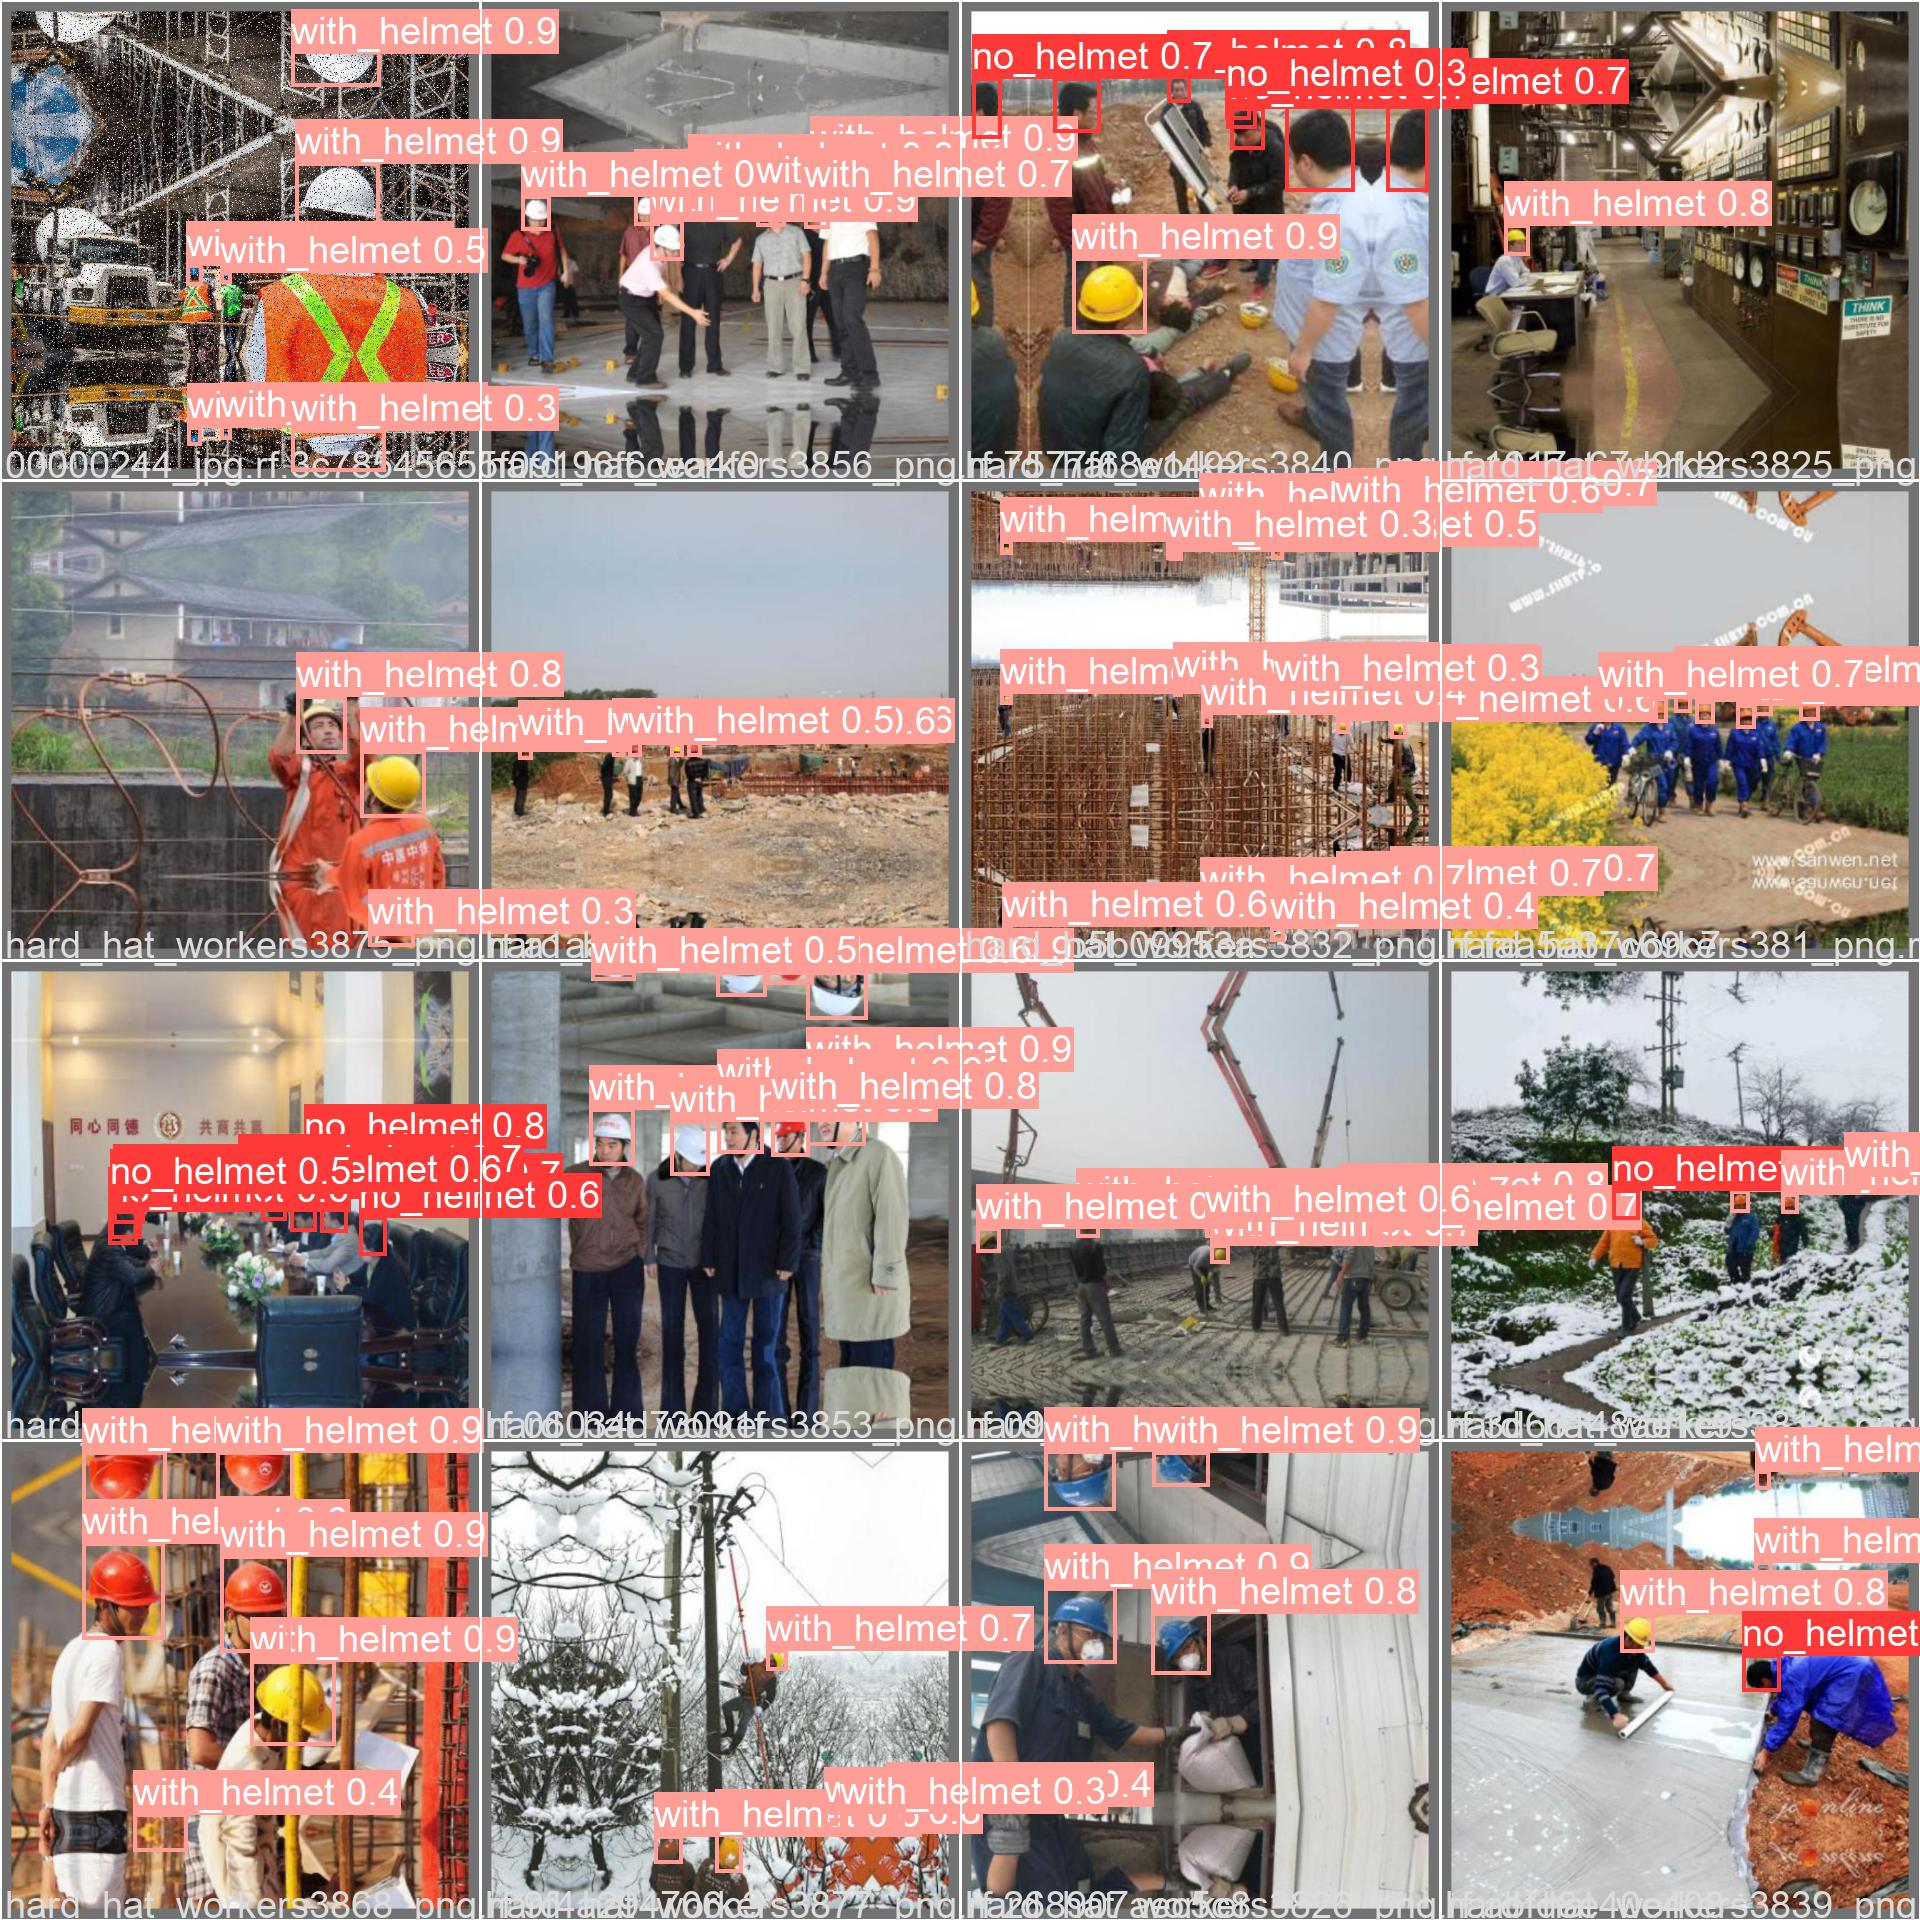
\includegraphics[scale=0.1]{gambar/train_v2_val/HelmetDetection_yolov5n2/val_batch0_pred.jpg}
  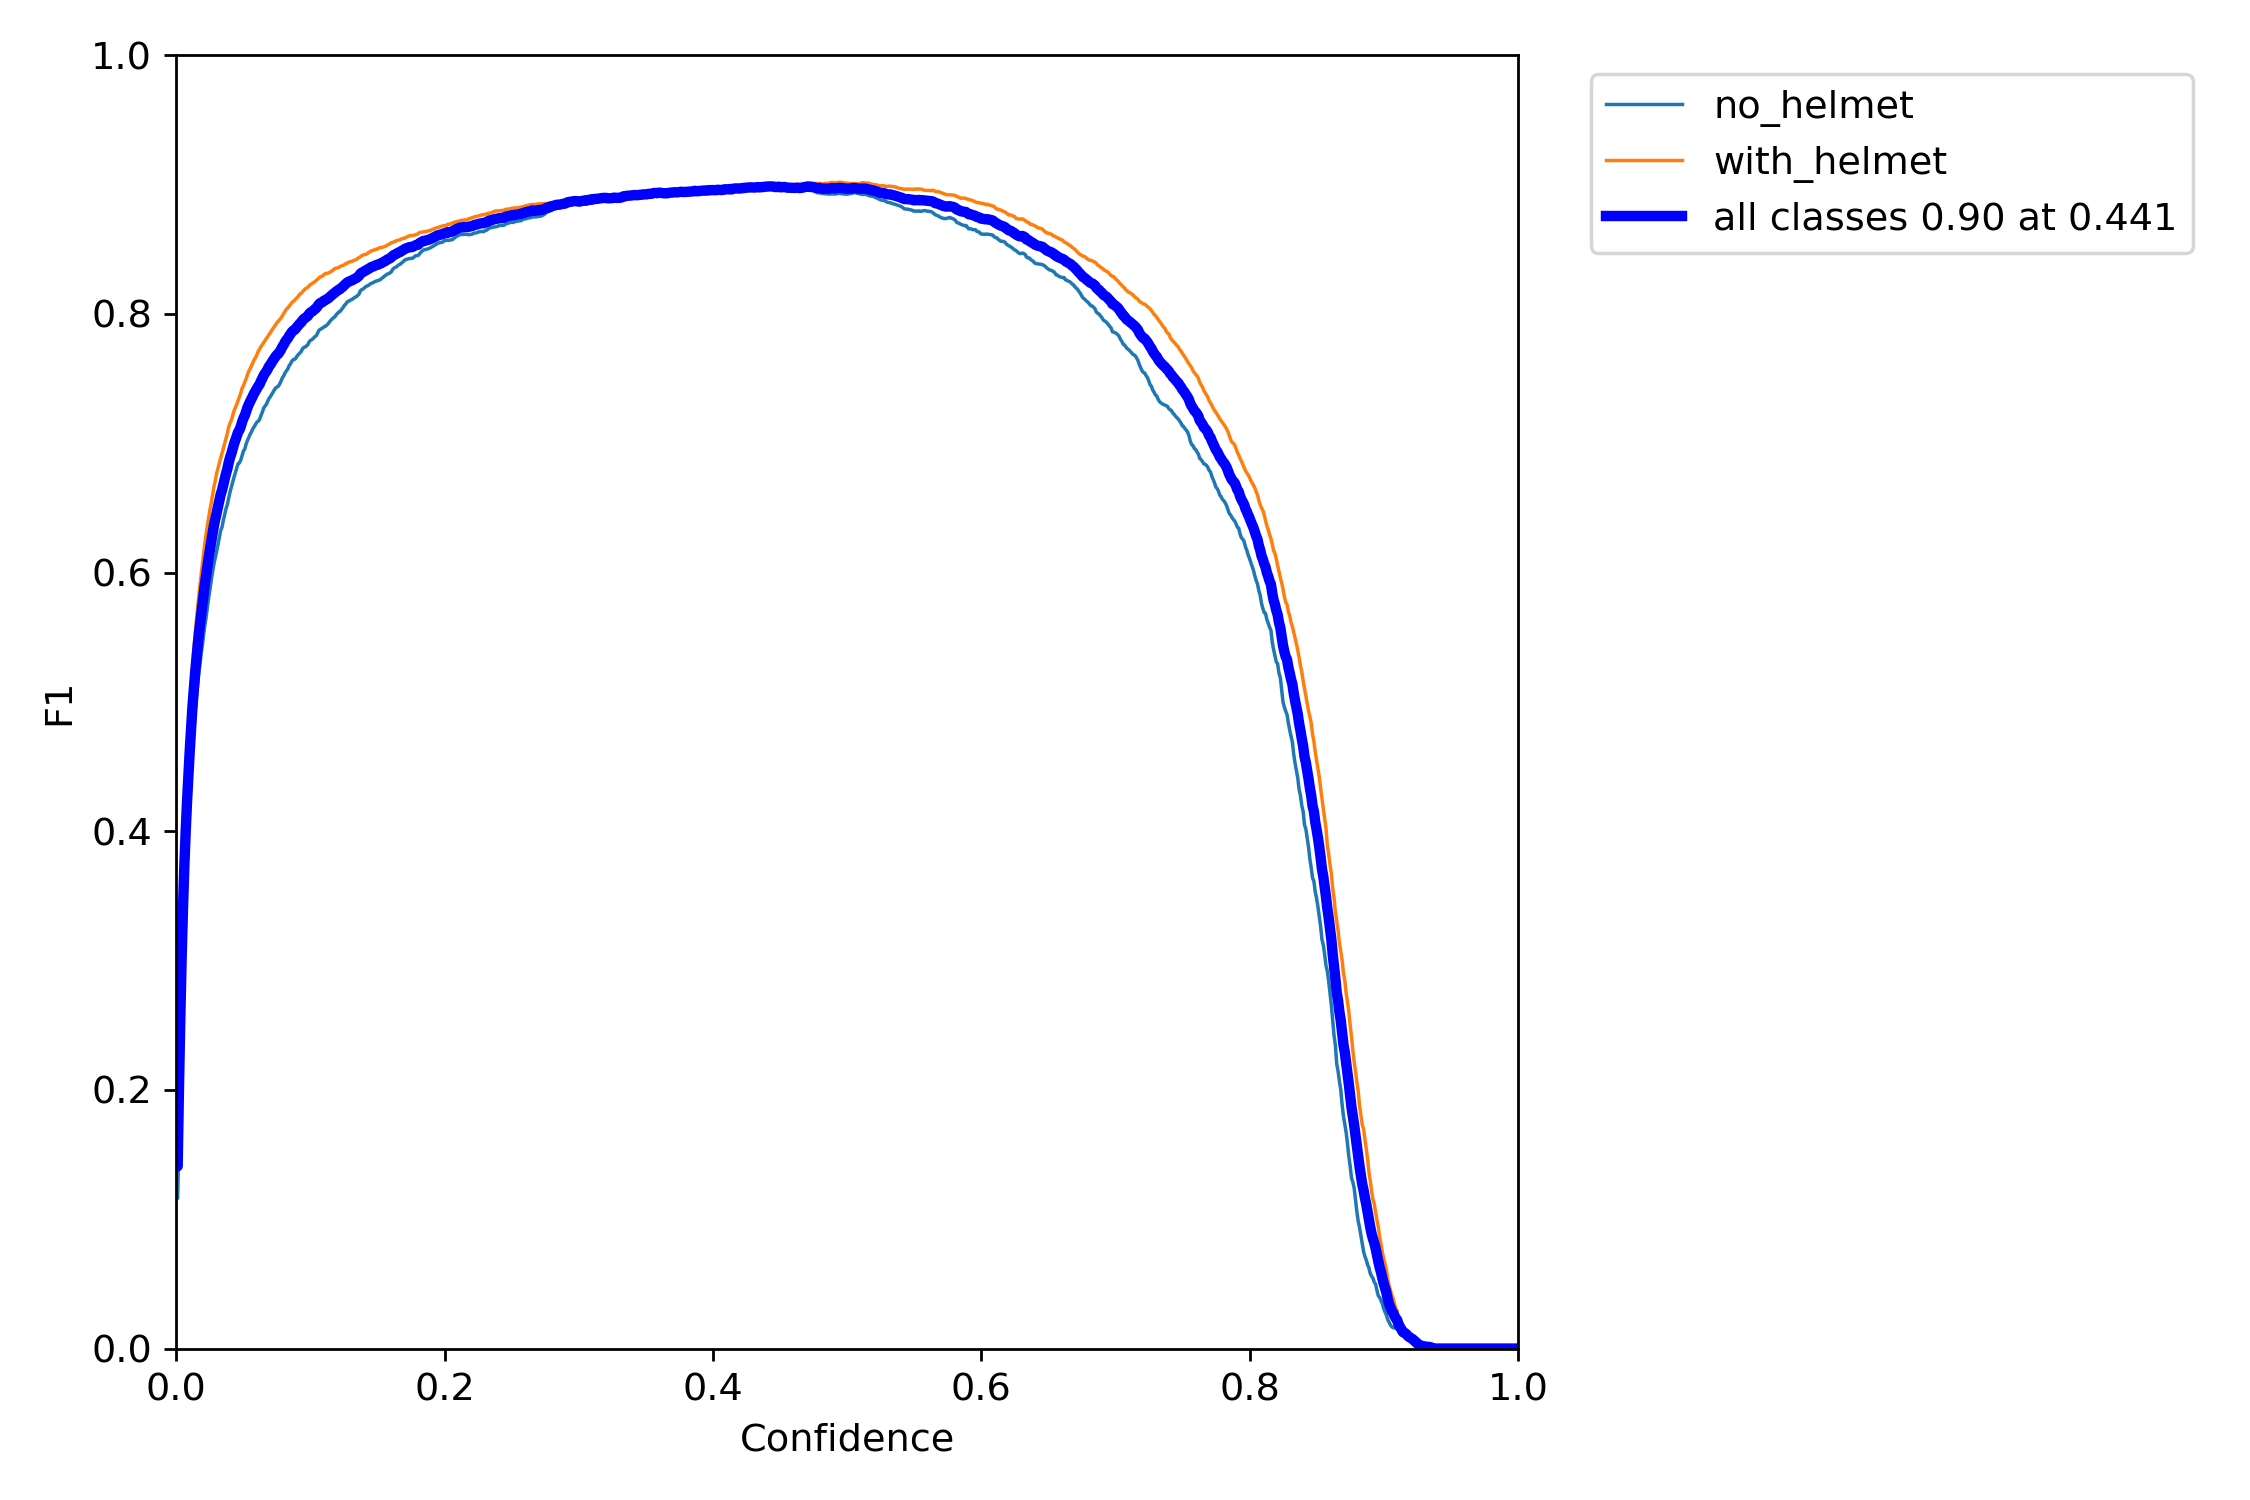
\includegraphics[scale=0.3]{gambar/train_v2_val/HelmetDetection_yolov5n2/F1_curve.png}
  \caption{Validasi Menggunakan Pretrain YOLOv5s}
  \label{fig:valyolov5n}  
\end{figure}

\subsection{Pengujian dengan Checkpoint \emph{YOLOv5s}}
\label{subsec:ujiyolo5s}

Pada pengujian ini.....

\begin{figure}[ht]
  \centering
  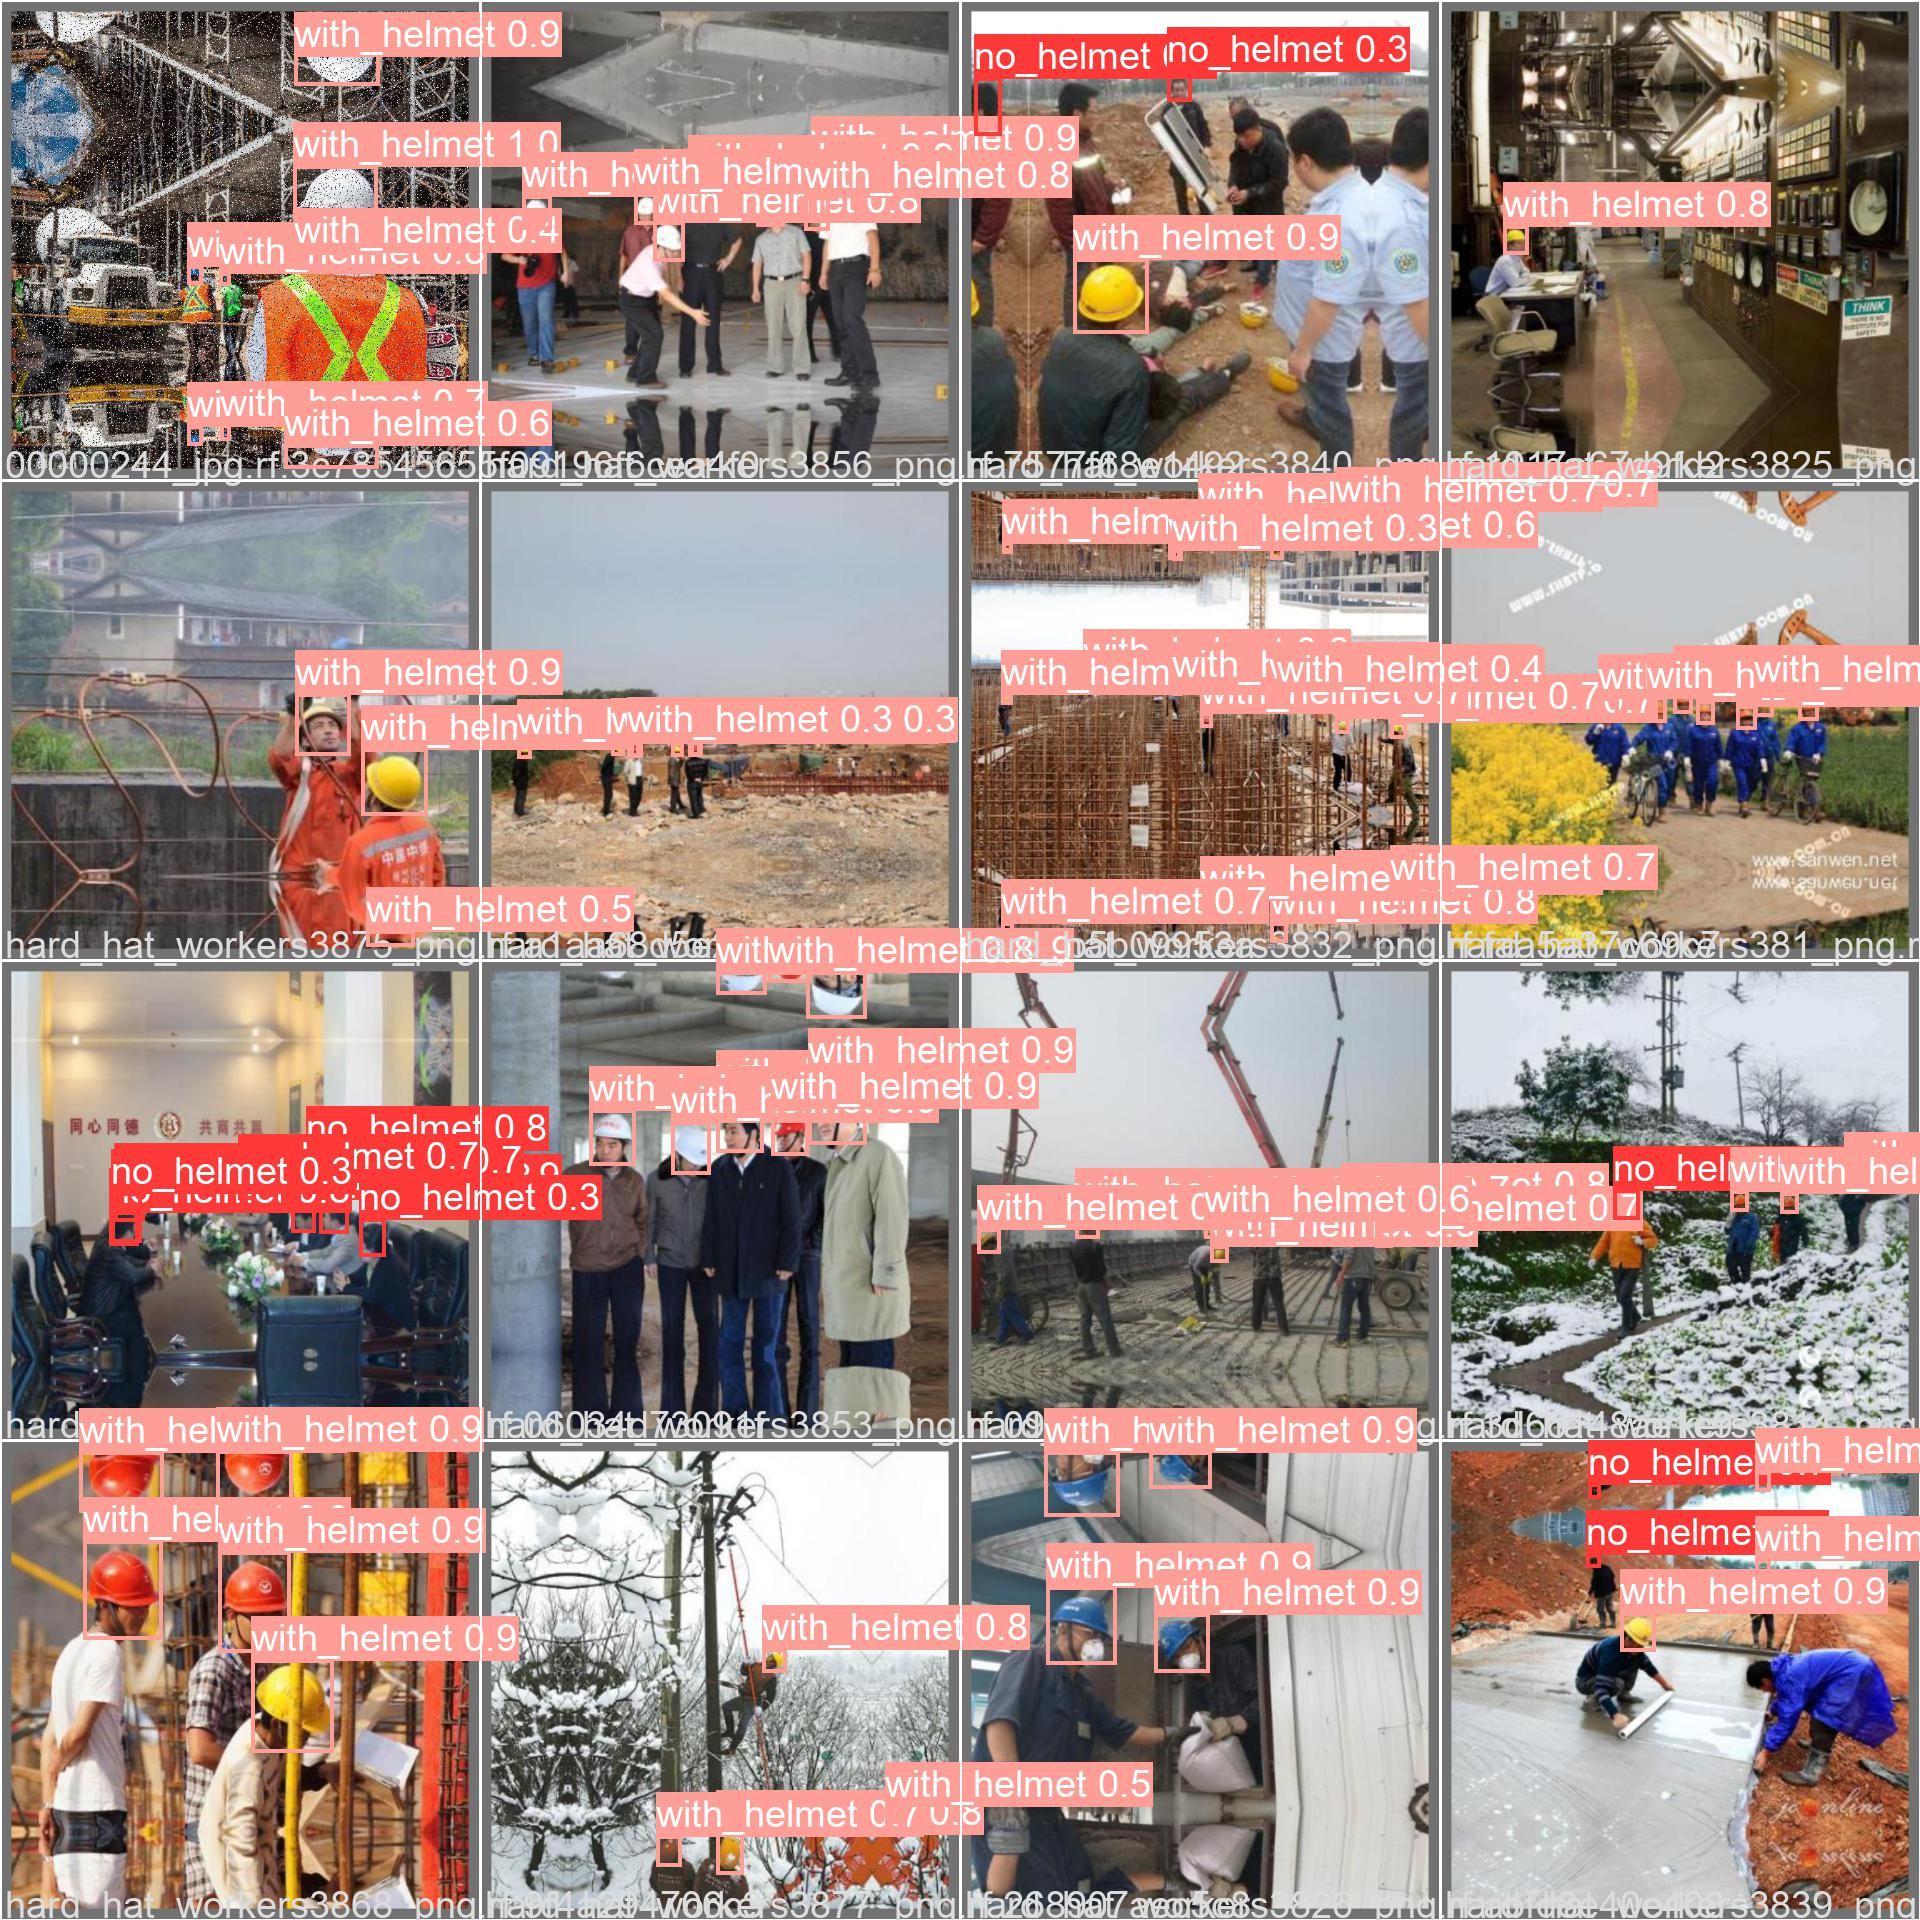
\includegraphics[scale=0.1]{gambar/train_v2_val/HelmetDetection_yolov5s/val_batch0_pred.jpg}
  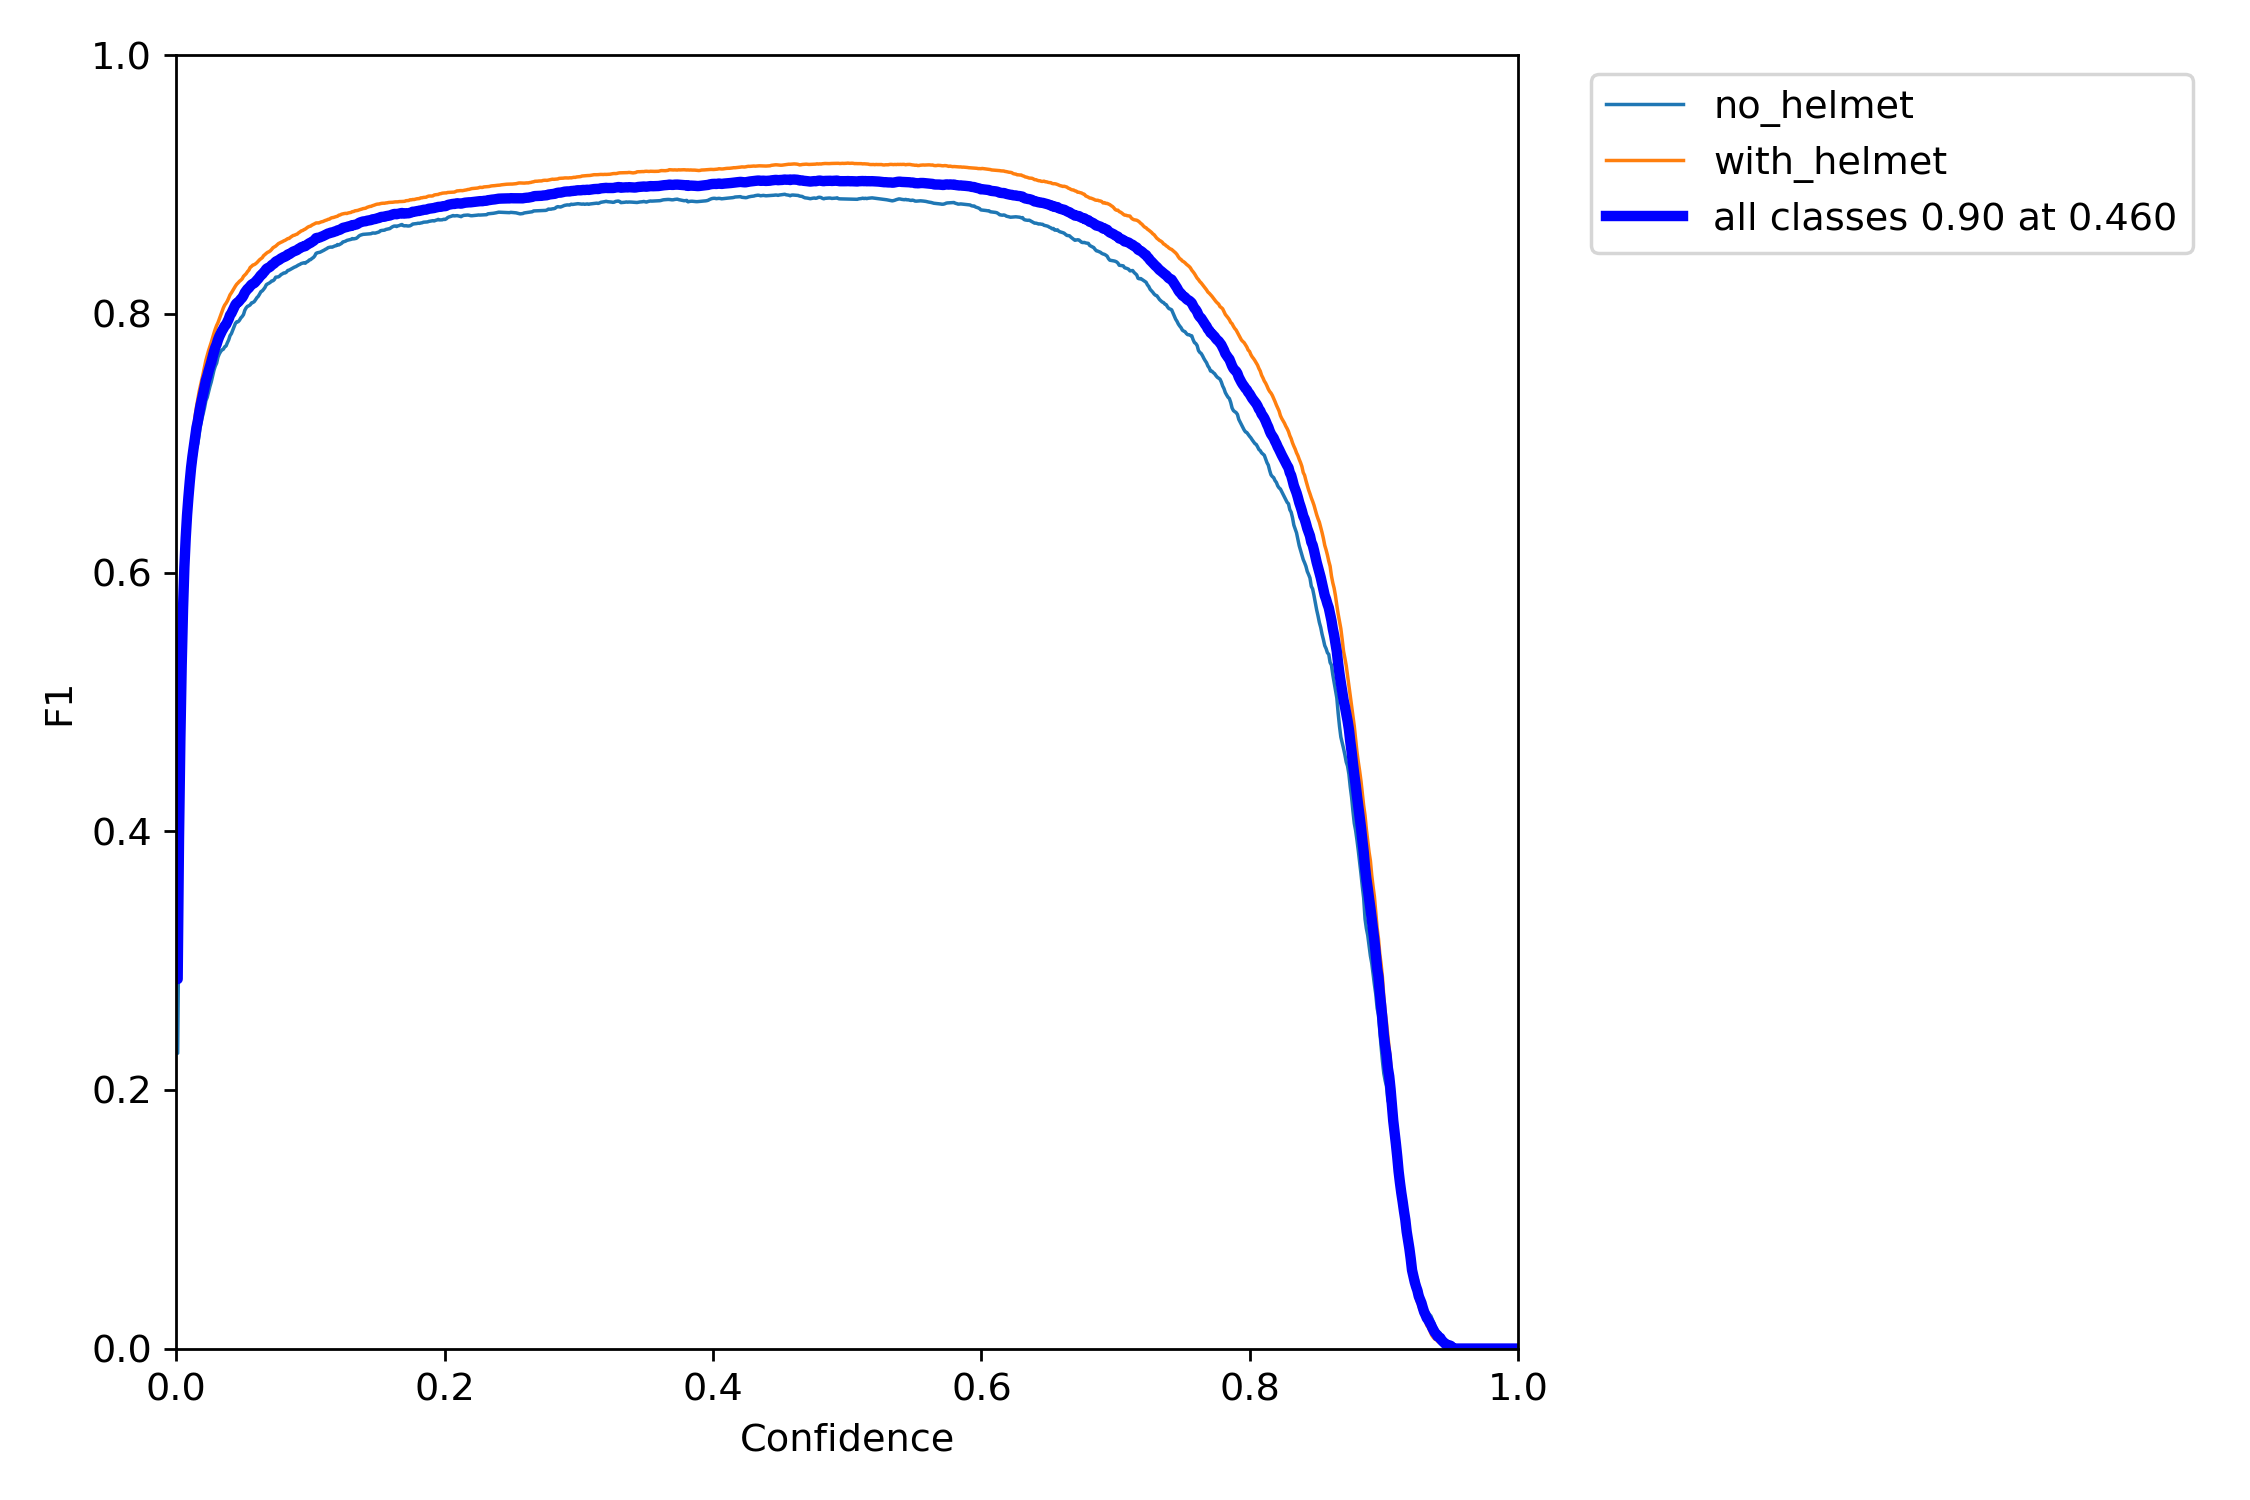
\includegraphics[scale=0.3]{gambar/train_v2_val/HelmetDetection_yolov5s/F1_curve.png}
  \caption{Validasi Menggunakan Pretrain YOLOv5s}
  \label{fig:valyolov5s}  
\end{figure}

\subsection{Pengujian dengan Checkpoint \emph{YOLOv5m}}
\label{subsec:ujiyolo5m}

Pada pengujian ini.....

\begin{figure}[ht]
  \centering
  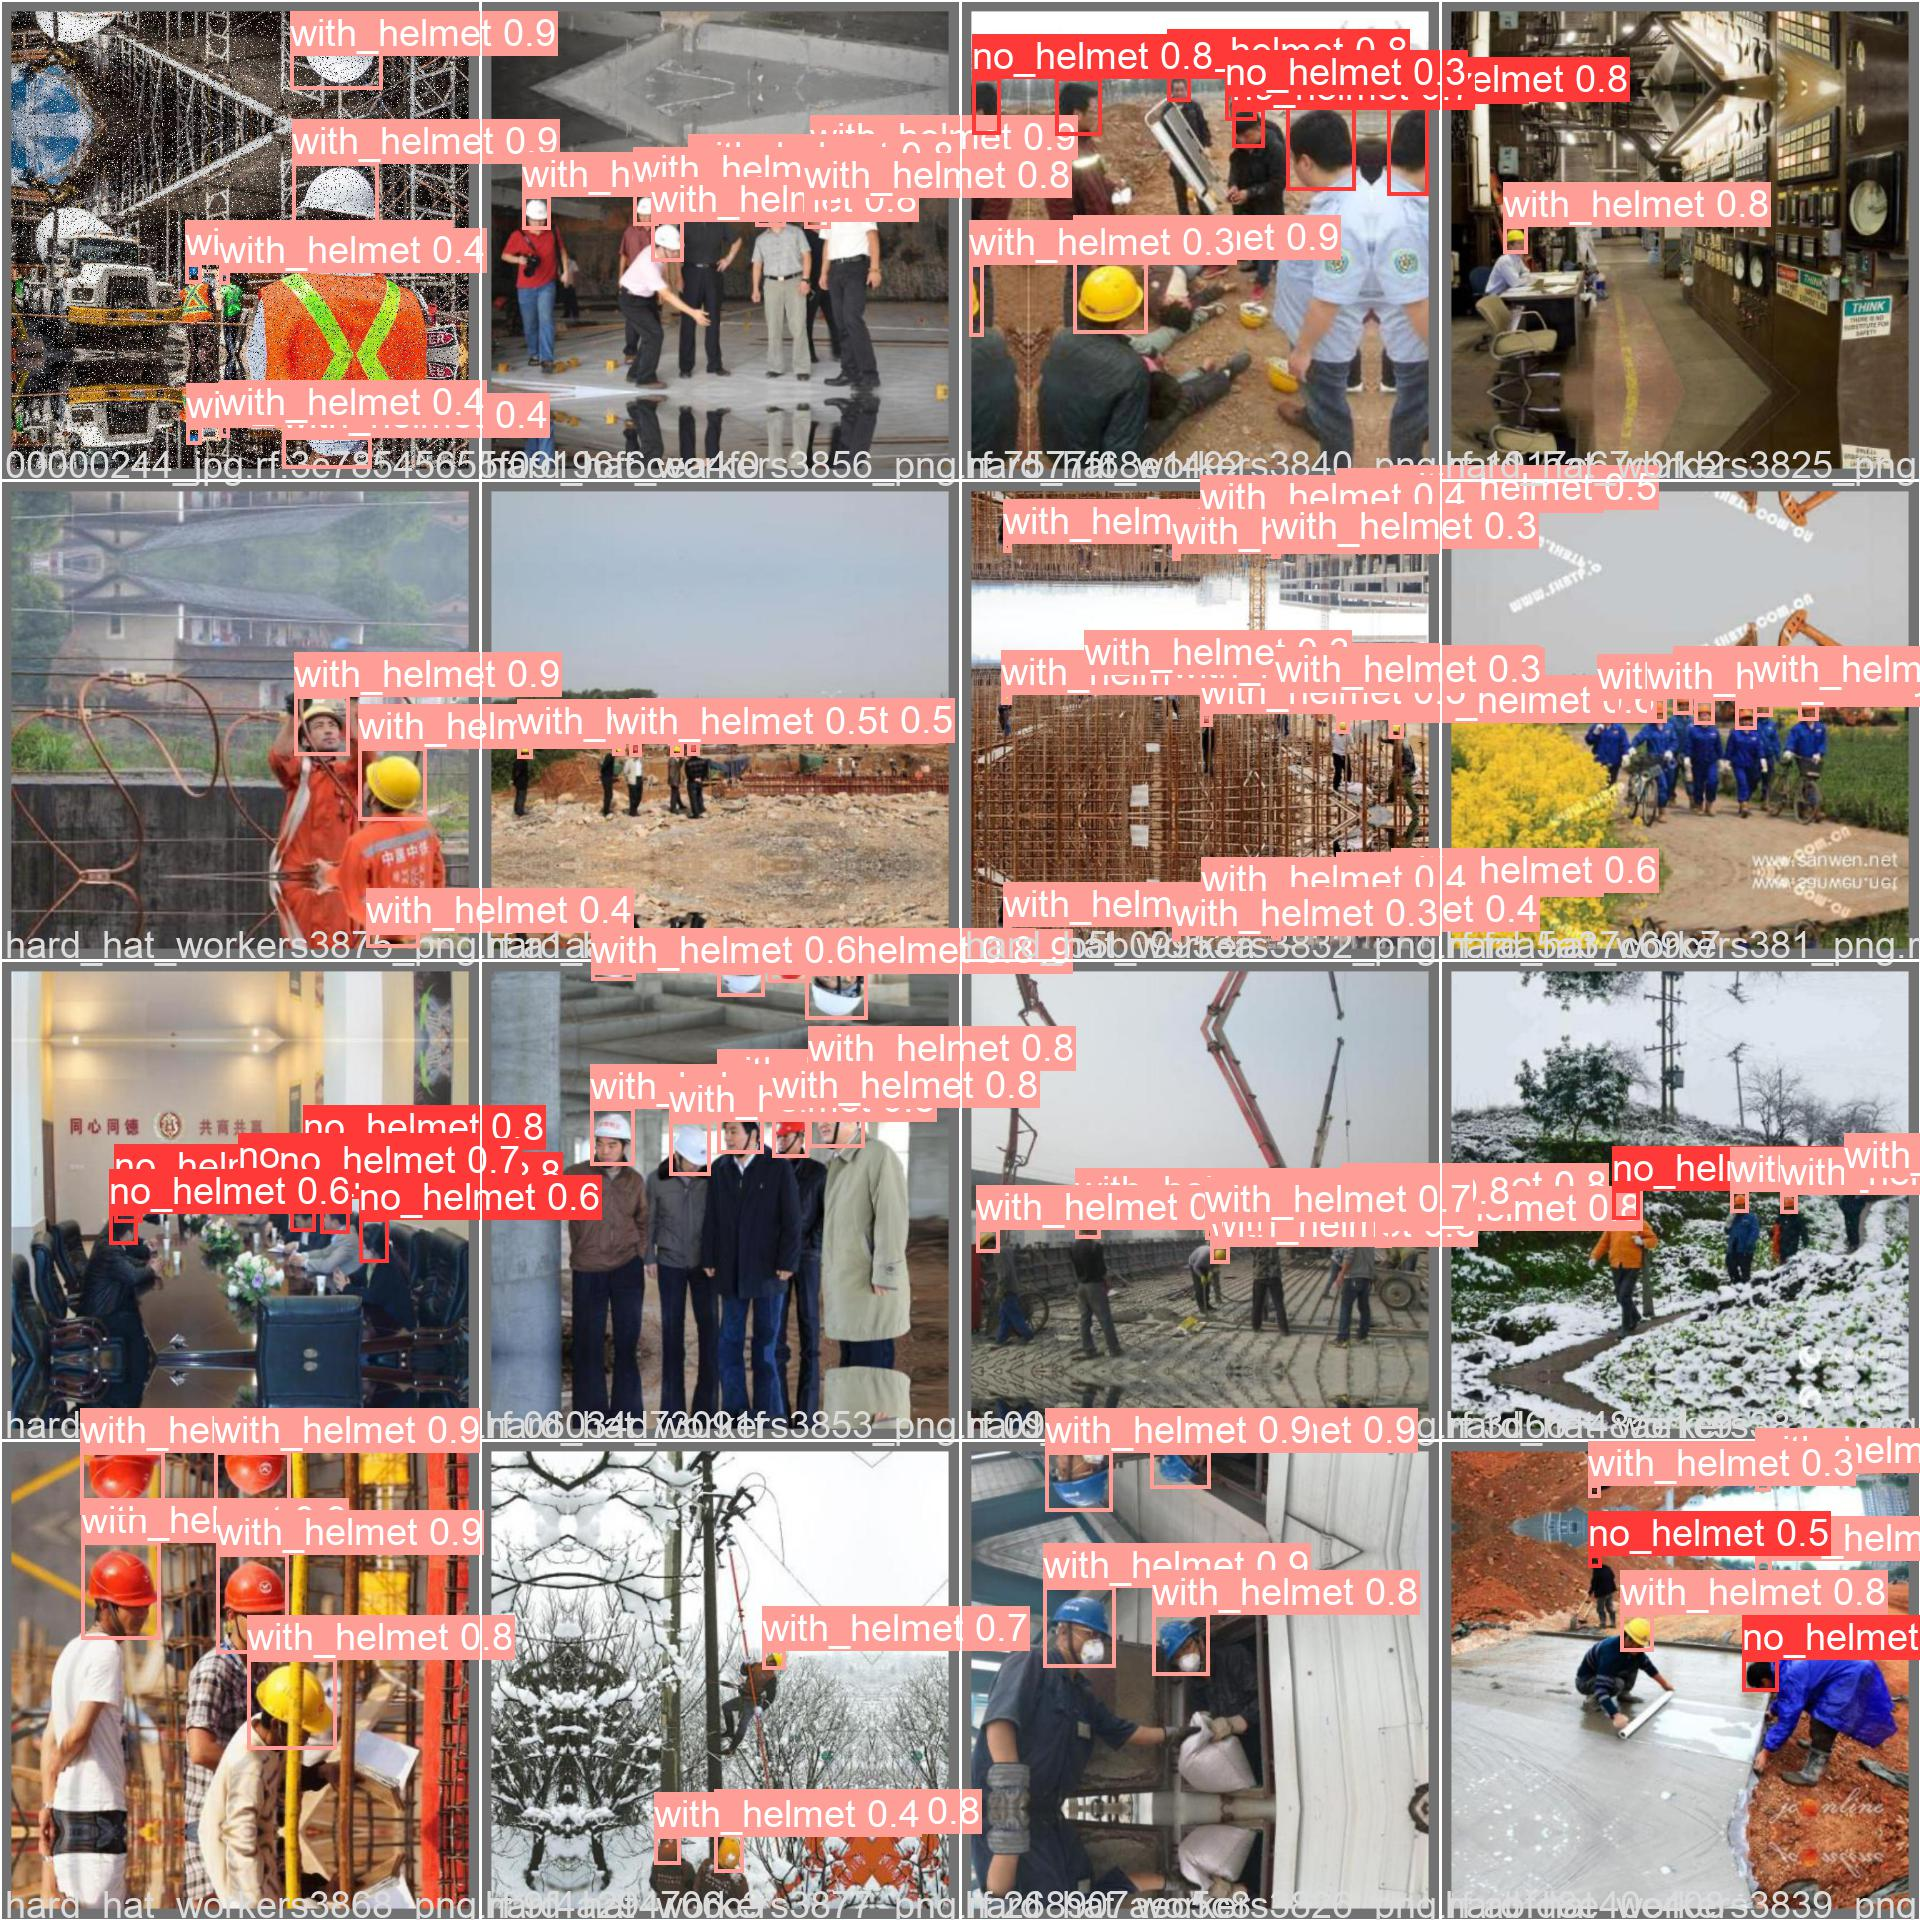
\includegraphics[scale=0.1]{gambar/train_v2_val/HelmetDetection_yolov5m/val_batch0_pred.jpg}
  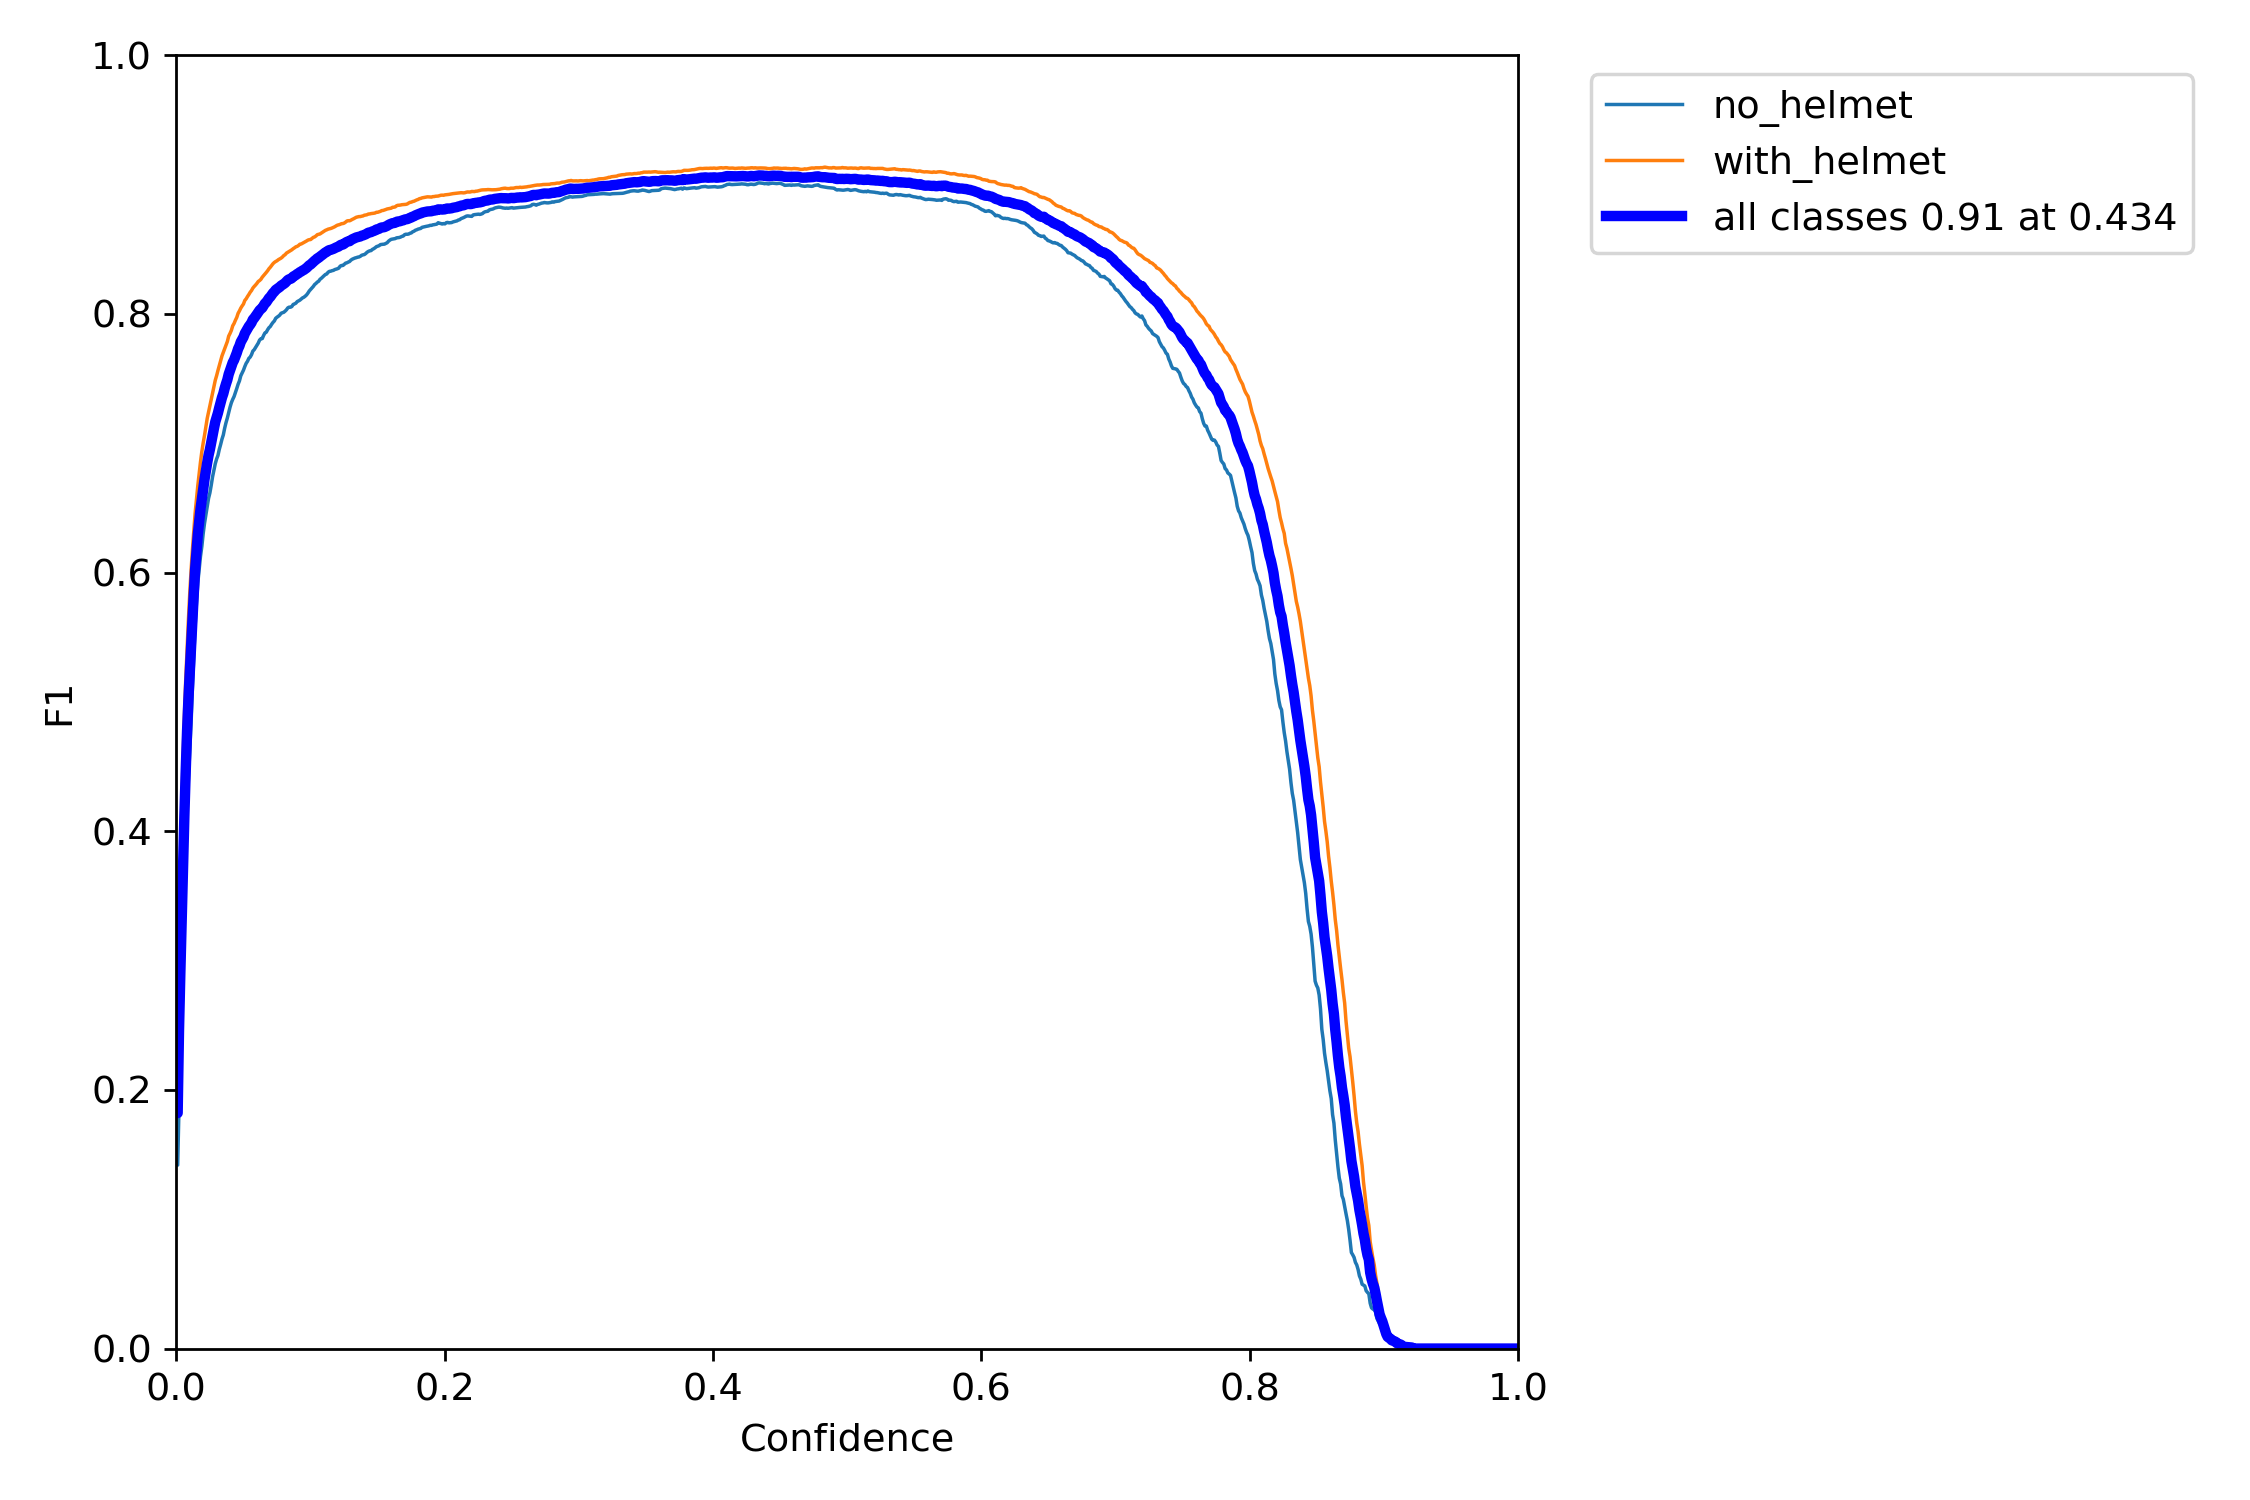
\includegraphics[scale=0.3]{gambar/train_v2_val/HelmetDetection_yolov5m/F1_curve.png}
  \caption{Validasi Menggunakan Pretrain YOLOv5m}
  \label{fig:valyolov5m}  
\end{figure}

\section{Pengujian Performa Berdasarkan Penggunaan Pretrain}
\label{sec:pengujianantarpretrain}

Pada bagian sebelumnya, digunakan pretrain yang sudah disediakan dari repository YOLOv5. Pada bagian ini dilakukan pengujian pada weight yang dibuat tanpa menggunakan pretrain yolov5 yang sudah disediakan dengan konfigurasi yang serupa dengan konfigurasi yolov5s.



\section{Evaluasi Pengujian}
\label{sec:analisispengujian}

Dari pengujian yang \lipsum[1]

% Contoh pembuatan tabel
\begin{longtable}{|c|c|c|}
  \caption{Hasil Pengukuran Energi dan Kecepatan}
  \label{tb:EnergiKecepatan}\\
  \hline
  \rowcolor[HTML]{C0C0C0}
  \textbf{Energi} & \textbf{Jarak Tempuh} & \textbf{Kecepatan} \\
  \hline
  10 J & 1000 M & 200 M/s \\
  20 J & 2000 M & 400 M/s \\
  30 J & 4000 M & 800 M/s \\
  40 J & 8000 M & 1600 M/s \\
  \hline
\end{longtable}

\lipsum[2-4]
